\subsection*{The weakness of a single layer}
    
        What can we do with a single layer? Well, our \textbf{LLC} model gives us an example: it has the \textbf{nonlinear} sigmoid activation, but acts as a \textbf{linear} separator.
        
        Why is that? Why is the separator still linear, if the \textbf{activation} isn't?
        
        Well, let's take the \textbf{linear} separator created by the pre-activation:
        
        \begin{equation}
            z = w^T x + w_0 = 0 
        \end{equation}
        
        This is our \textbf{boundary} for just a linear function. But adding the nonlinear activation should make it more \textbf{complex}, right? 
        
        Well, it turns out, we can represent our \textbf{activation} boundary with a \textbf{linear} boundary.
        
        \miniex Continue our LLC example. If $z=0$, then $\sigma(z) = \sigma(0)$. Our boundary is
        
        \begin{equation}
            \sigma(z)=\sigma(0)=\frac{1}{2}
        \end{equation}
        
        Wait. But that means that $\sigma(z)=.5$ is the same as $z=0$: the same inputs $x$ cause both of them, so they have the same boundary!
        
        \begin{equation}
            \text{Linear boundary } z=0 \Longleftrightarrow f(z)=\frac{1}{2}
        \end{equation}
        
        Summary:
        
        \begin{itemize}
            \item $\sigma(z)=.5$ is the \textbf{same} as $z=0$.
            \item $z=0$ is \textbf{linear}.
            \item Thus, our sigmoid boundary is \textbf{linear}.
        \end{itemize}
        
        We can apply this to other activation functions. In general, any constant boundary for most $f(z)$ is equivalent to some linear boundary $z=C$:
            \note{Assuming that $f$ is invertible, which it often is.}
        
        \begin{equation}
            z=C 
            \qquad
            \Longleftrightarrow
            \qquad
            f(z)=f(C)
        \end{equation}
        
        Since $z=C$ is linear, we know that our activation separator $f(x)=f(C)$ is linear too.\\
        
        \begin{concept}
            A single neuron creates a \vocab{linear separator}, even if it has a \purp{nonlinear} activation.
            
            This is because any \gren{boundary} for $f(z)$ we can create, can be represented by some \purp{linear} boundary in $z$.
        \end{concept}
        
            \note{There are exceptions, but this is true for most useful activation functions.}
        
        It turns out, adding more neurons \textbf{within} the layer doesn't change much: because they act in \textbf{parallel}, each neuron acts separately, and the things we said above are still \textbf{true} for each output $a_i$.
        
        \begin{figure}[H]
            \centering
            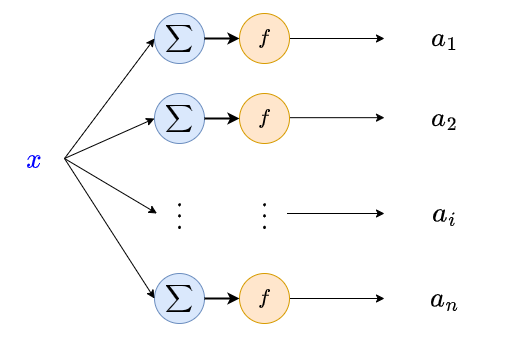
\includegraphics[width=80mm,scale=0.4]{images/nn_images/remove_input.png}
            \caption*{Each of these neurons has the same input, $x$.}
        \end{figure}
        
        So, in order to create nonlinear behavior, we need at least two layers of neurons in \textbf{series}.
        
        So, we'll start \textbf{stacking} layers on each other: each layer \textbf{feeds} into the next one.\\
        
        \begin{concept}
            A \vocab{single layer} of neurons has \gren{linear} behavior.
            
            We need \gren{multiple} layers to get a nonlinear \purp{neural network}.
        \end{concept}